\chapter{Estado del arte}
\label{ch:arte}

Antes de abordar los detalles del trabajo, conviene situar el problema en su contexto teórico. La predicción de series temporales financieras tiene una trayectoria prolongada ---desde la metodología Box-Jenkins en los años 70 hasta las redes neuronales actuales--- y ha evolucionado desde modelos estadísticos clásicos hacia enfoques de aprendizaje automático de complejidad creciente~\cite{sezer2020financial}. En este capítulo se revisan los fundamentos necesarios para comprender la metodología adoptada.

\section{Peculiaridades de las series temporales financieras}

Las series financieras presentan propiedades que las distinguen de otras series temporales de carácter físico o demográfico. Su comportamiento difiere del de series como la temperatura o la población: exhiben una volatilidad irregular, experimentan cambios de régimen sin previo aviso y, a diferencia de muchas series naturales, carecen de estacionalidades estables. Todo ello condiciona tanto el diseño de los modelos como la forma de evaluarlos.

\subsection{El ruido como protagonista}

Una característica recurrente en datos financieros a corto plazo es el ruido~\cite{cont2001empirical}. Las variaciones diarias reflejan miles de decisiones de agentes que operan con información incompleta, estados de ánimo distintos y horizontes diferentes. El resultado es una señal en la que resulta difícil distinguir un patrón real de una coincidencia estadística.

La consecuencia práctica es que patrones aparentemente claros en retrospectiva pueden no sostenerse fuera de muestra. El sobreajuste constituye uno de los principales riesgos en predicción financiera~\cite{sezer2020financial}: un modelo que memoriza el pasado ofrecerá resultados excelentes en entrenamiento pero mediocres en predicción real.

\subsection{La no estacionariedad}

Los precios tienden a mostrar no estacionariedad: el nivel medio puede desplazarse de forma persistente y la distribución de rendimientos cambia con el tiempo. Esta propiedad complica el uso directo de técnicas que asumen parámetros constantes.

Por eso es habitual trabajar con rendimientos en lugar de precios absolutos. El rendimiento logarítmico entre dos días consecutivos,
\[
r_t = \ln\left(\frac{P_t}{P_{t-1}}\right),
\]
tiene propiedades estadísticas más manejables y permite comparar activos con escalas de precio muy diferentes.

\subsection{Los hechos estilizados}

A pesar del ruido y la aparente aleatoriedad, las series financieras exhiben ciertas regularidades empíricas que se observan de manera consistente en mercados muy diversos~\cite{cont2001empirical}. Los investigadores las llaman \emph{hechos estilizados}:

La \textbf{agrupación de volatilidad} es quizá la más conocida. Los episodios de alta volatilidad tienden a agruparse en el tiempo, al igual que los periodos de calma. Este fenómeno tiene implicaciones importantes para la gestión del riesgo y motivó el desarrollo de modelos como ARCH/GARCH~\cite{engle1982autoregressive, bollerslev1986generalized}.

Las \textbf{colas pesadas} de las distribuciones de rendimientos son otro hecho ampliamente documentado en la literatura~\cite{mandelbrot1963variation, cont2001empirical}. Los eventos extremos ---caídas del 10\% en un día que según la distribución normal deberían ocurrir una vez cada varios siglos--- suceden con una frecuencia notablemente superior a la esperada. Cualquier modelo que asuma normalidad estará subestimando el riesgo real.

También existe el llamado \textbf{efecto apalancamiento}: las caídas de precio suelen ir acompañadas de aumentos de volatilidad mayores que las subidas~\cite{cont2001empirical}. Esta asimetría se ha observado de forma consistente en distintos mercados.

\section{La hipótesis de los mercados eficientes}

La Hipótesis de los Mercados Eficientes, formulada por Fama en 1970~\cite{fama1970efficient}, sostiene que los precios reflejan la información disponible, de modo que obtener ventajas sistemáticas de forma consistente resulta, cuando menos, difícil.

La versión más débil de esta hipótesis dice que los precios pasados no contienen información útil para predecir el futuro ---lo que invalidaría todo el análisis técnico---. Versiones más fuertes afirman que ni siquiera los estados financieros públicos o la información privilegiada permitirían obtener rendimientos superiores.

La evidencia empírica es mixta. Por un lado, la mayoría de los gestores activos de fondos no consiguen batir a los índices de referencia de forma consistente. Por otro lado, existen anomalías documentadas (el efecto momentum, el efecto valor, ciertos patrones estacionales) que sugieren ineficiencias explotables. Este trabajo parte de la premisa de que existe cierto grado de predictibilidad, aunque sea modesto y difícil de capturar.

\section{Los modelos estadísticos clásicos}

Durante décadas, los modelos ARIMA fueron la herramienta de referencia para analizar series temporales. La metodología Box-Jenkins, desarrollada en los años 70~\cite{box2015time}, propone un proceso iterativo para identificar el orden apropiado del modelo, estimar sus parámetros y verificar que los residuos se comportan como ruido blanco.

Un modelo ARIMA$(p,d,q)$ tiene tres componentes: $p$ términos autorregresivos (el precio depende de sus valores pasados), $d$ diferenciaciones (para lograr estacionariedad) y $q$ términos de media móvil (que capturan la persistencia de los shocks). En la práctica, un modelo simple como ARIMA$(5,1,0)$ ---cinco retardos autorregresivos y una diferenciación--- ya captura buena parte de la dinámica a corto plazo.

Junto con ARIMA, en práctica aplicada se utiliza con frecuencia un baseline \emph{naive}: asumir que la mejor predicción para $t+h$ es el último cierre observado en $t$. Aunque es un enfoque muy simple, en series financieras de corto plazo suele ser sorprendentemente competitivo y por eso se adopta habitualmente como referencia mínima en comparativas de modelos.

Estos modelos tienen la ventaja de ser interpretables y de contar con una teoría estadística bien desarrollada. Su limitación principal es que asumen relaciones lineales, lo que puede ser restrictivo en mercados donde las no linealidades abundan.

\section{El auge del aprendizaje automático}

El aprendizaje automático plantea un enfoque diferente: en lugar de imponer una forma funcional concreta, se ajustan modelos flexibles guiados por los datos~\cite{lecun2015deep}. Algoritmos como Random Forest~\cite{breiman2001random} o XGBoost~\cite{chen2016xgboost} pueden capturar relaciones no lineales sin necesidad de definirlas explícitamente.

Random Forest construye múltiples árboles de decisión sobre submuestras de los datos y promedia sus predicciones. Tiende a ser robusto y proporciona medidas de importancia de variables. XGBoost extiende este enfoque mediante \textit{boosting} secuencial, donde cada nuevo árbol corrige los errores del conjunto anterior. Por su rendimiento, se ha adoptado ampliamente en aplicaciones prácticas y en entornos de competición.

Una limitación es que estos modelos no están diseñados específicamente para series temporales. No incorporan de forma nativa el orden temporal ni las dependencias entre observaciones, por lo que requieren una etapa de ingeniería de características: creación de retardos, cálculo de indicadores técnicos~\cite{murphy1999technical} y estadísticas rodantes. La calidad de estas características condiciona en gran medida el rendimiento final.

\section{Las redes neuronales recurrentes}

Las redes recurrentes abordan el problema de la temporalidad de forma directa. En lugar de recibir un vector fijo de características, procesan los datos como una secuencia, manteniendo una memoria interna que se actualiza en cada paso temporal. Esto les permite, en principio, aprender dependencias de largo alcance sin necesidad de especificarlas manualmente.

El problema es que las redes recurrentes tradicionales sufren del desvanecimiento del gradiente: al retropropagar errores a través de muchos pasos temporales, los gradientes tienden a hacerse insignificantes, impidiendo que la red aprenda dependencias lejanas. Las arquitecturas LSTM~\cite{hochreiter1997long} y GRU~\cite{cho2014learning} resuelven este problema mediante mecanismos de puertas que controlan el flujo de información.

La Figura~\ref{fig:lstm_vs_gru} compara ambas arquitecturas.

\begin{figure}[H]
\centering
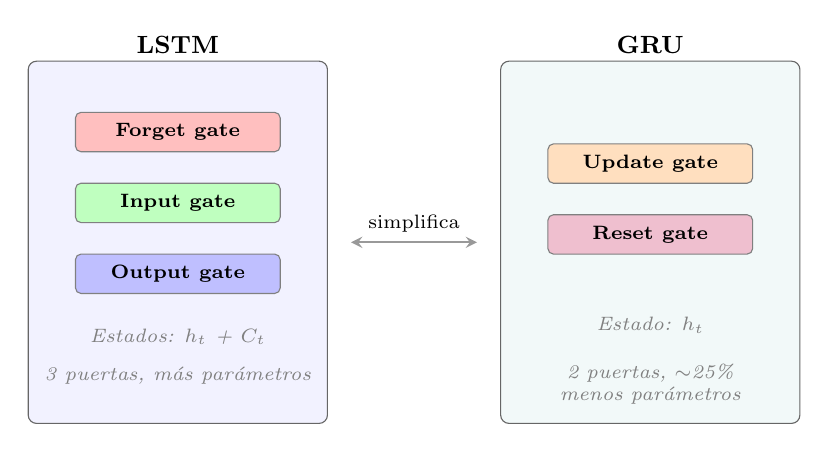
\begin{tikzpicture}[
  cell/.style={rectangle, rounded corners=3pt, draw=black!60, minimum width=3.8cm, minimum height=4.6cm, fill=#1!5},
  gate/.style={rectangle, rounded corners=2pt, draw=black!50, fill=#1!25, minimum width=2.6cm, minimum height=0.5cm, font=\scriptsize\bfseries, text centered},
  lbl/.style={font=\small\bfseries},
  sublbl/.style={font=\scriptsize\itshape, text=black!50}
]
  % LSTM cell
  \node[cell=blue] (lstm) at (0,0) {};
  \node[lbl] at (0,2.5) {LSTM};
  \node[gate=red]   at (0,1.4)  {Forget gate};
  \node[gate=green] at (0,0.5)  {Input gate};
  \node[gate=blue]  at (0,-0.4) {Output gate};
  \node[sublbl] at (0,-1.2) {Estados: $h_t$ + $C_t$};
  \node[sublbl] at (0,-1.7) {3 puertas, más parámetros};

  % GRU cell
  \node[cell=teal] (gru) at (6,0) {};
  \node[lbl] at (6,2.5) {GRU};
  \node[gate=orange] at (6,1.0)  {Update gate};
  \node[gate=purple] at (6,0.1)  {Reset gate};
  \node[sublbl] at (6,-1.05) {Estado: $h_t$};
  \node[sublbl, align=center, text width=2.7cm] at (6,-1.80) {2 puertas, $\sim$25\%\\menos parámetros};

  % Flecha comparativa
  \draw[<->, >=stealth, thick, draw=black!40] (2.2,0) -- node[above, font=\scriptsize] {simplifica} (3.8,0);
\end{tikzpicture}
\caption{Comparación entre arquitecturas LSTM y GRU.}
\label{fig:lstm_vs_gru}
\end{figure}

Una celda LSTM decide en cada paso qué información olvidar del estado anterior, qué información nueva incorporar y qué parte del estado usar como salida. Esta capacidad de retener selectivamente información relevante durante largos periodos es lo que hace a las LSTM especialmente adecuadas para series temporales~\cite{fischer2018deep}.

La GRU simplifica la arquitectura de la LSTM combinando algunas puertas. Tiene menos parámetros y suele converger más rápido, con resultados a menudo comparables. En la práctica, la elección entre LSTM y GRU suele determinarse empíricamente en función del conjunto de datos y del compromiso entre capacidad y complejidad.

La Figura~\ref{fig:lstm_vs_gru} resume las diferencias clave entre ambas arquitecturas. En ella se aprecia que LSTM emplea tres puertas (olvido, entrada y salida) y mantiene dos estados internos separados ($h_t$ para la salida y $C_t$ para la memoria de largo plazo), lo que le confiere una mayor capacidad para modelar dependencias temporales muy extensas. Por contra, GRU reduce la complejidad a dos puertas (reset y update) y un único estado oculto, lo que se traduce en menos parámetros, entrenamientos más rápidos y menor riesgo de sobreajuste en datasets pequeños. Ambas arquitecturas resuelven el problema del desvanecimiento del gradiente y son ampliamente utilizadas en predicción de series temporales financieras~\cite{fischer2018deep}.

\textbf{CNN 1D en series temporales.} Además de las arquitecturas recurrentes, en predicción de series temporales se emplean también redes convolucionales unidimensionales (CNN 1D). Una CNN 1D aplica filtros sobre el eje temporal y puede aprender patrones locales (por ejemplo, combinaciones de cambios en ventanas cortas de días consecutivos). Su principal ventaja es que suele entrenar más rápido y con menos parámetros que una recurrente. Como contrapartida, si su campo receptivo efectivo es pequeño, puede capturar peor dependencias de largo plazo que LSTM/GRU. En este trabajo se evalúa una CNN 1D como alternativa más ligera para valorar si los patrones locales resultan suficientes o si es necesario un mecanismo explícito de memoria.

\section{Transformers en series temporales}

Los Transformers~\cite{vaswani2017attention} han pasado a ser una arquitectura de referencia en problemas secuenciales gracias al mecanismo de autoatención, que permite modelar dependencias de largo alcance sin recurrencia. En series temporales, se han propuesto variantes adaptadas a \textit{forecasting} multi-horizonte y a secuencias largas. Un ejemplo es el \emph{Temporal Fusion Transformer}~\cite{lim2021tft}, que combina autoatención con componentes de interpretabilidad y maneja predicción multi-horizonte. Otro ejemplo es \emph{Informer}~\cite{zhou2021informer}, diseñado para mejorar la eficiencia en secuencias largas mediante mecanismos de atención aproximada.

No obstante, la evidencia reciente sugiere que los Transformers no garantizan mejoras sistemáticas en todos los escenarios: su rendimiento depende del tamaño del conjunto de datos, la calidad de la señal y un ajuste cuidadoso. En particular, se ha observado que, en ciertos benchmarks de predicción, modelos más simples pueden igualar o superar a arquitecturas basadas en atención~\cite{zeng2023transformers}. Esta discusión es relevante en finanzas, donde el número de observaciones suele ser limitado y la no estacionariedad es elevada.

\section{El sentimiento como variable predictiva}

Hasta aquí se ha considerado la predicción a partir de precios pasados. Sin embargo, los mercados también reaccionan a noticias, informes y decisiones macroeconómicas. Incorporar información externa puede aportar poder predictivo adicional, aunque su utilidad depende del activo y del horizonte temporal.

El análisis de sentimiento intenta cuantificar el tono del flujo de información que llega al mercado. Puede realizarse con enfoques basados en diccionarios o con modelos de lenguaje entrenados o adaptados al dominio financiero~\cite{liu2020finbert}. Bollen et al.~\cite{bollen2011twitter} mostraron de forma temprana que el sentimiento agregado en redes sociales podía anticipar movimientos del índice Dow Jones, y Baker y Wurgler~\cite{baker2007investor} sintetizan la relevancia del sentimiento desde una perspectiva de finanzas empíricas.

Existen también índices de sentimiento ya calculados que agregan múltiples fuentes. Algunos intentan medir el clima general del mercado y otros se centran en activos concretos a partir de noticias y cobertura mediática. En este trabajo se optó por GDELT, que permite construir series diarias de tono medio por consulta, sin clave y con histórico amplio~\cite{gdelt2024api}.

La idea de combinar información histórica de precios con señales de sentimiento constituye el elemento central de este trabajo. La hipótesis es que ambas fuentes de información son complementarias: los precios pasados capturan la dinámica interna del mercado, mientras que el sentimiento refleja factores externos que pueden anticipar cambios de régimen.

\section{Cómo evaluar las predicciones}

Medir el éxito de un modelo de predicción requiere elegir métricas apropiadas. Para tareas de regresión, las más habituales son el error cuadrático medio (RMSE), el error absoluto medio (MAE) y el error porcentual medio absoluto (MAPE)~\cite{hyndman2006another}:

\[
\text{RMSE} = \sqrt{\frac{1}{n}\sum_{i=1}^{n}(y_i - \hat{y}_i)^2}, \quad
\text{MAE} = \frac{1}{n}\sum_{i=1}^{n}|y_i - \hat{y}_i|, \quad
\text{MAPE} = \frac{100}{n}\sum_{i=1}^{n}\left|\frac{y_i - \hat{y}_i}{y_i}\right|
\]

El RMSE penaliza especialmente los errores grandes, lo que puede ser apropiado o no dependiendo del contexto. El MAE es más robusto ante valores atípicos. El MAPE expresa el error como porcentaje, lo que facilita la comparación entre activos con escalas de precio muy diferentes ---un error de 100 dólares resulta significativo para una acción valorada en 50 dólares, pero insignificante para Bitcoin---.

En este trabajo se utiliza el MAPE como métrica principal de comparación, complementado con RMSE y MAE para dar una visión más completa. Además, al tratarse de predicción direccional, se incorporan métricas propias de clasificación: el acierto direccional (MDA), el F1 direccional y el MCC, que es más robusto ante desequilibrios entre subidas y bajadas.
